\chapter{Newton polygons}
	We'll now introduce a very useful tool to study radius of convergence and zeroes of an analytic function: the Newton polygon. We'll first introduce it for polynomials and then try to generalize our results to power series.
	\section{Newton polygons for polynomials}
		\begin{defn}
			\label{defn:newton-polygon-polynomials}
			Let $f(X) = 1 + \sum_{i=1}^n a_iX^i \in 1 + X\Cp[X]$ be a polynomial and consider the following set of points in $\R^2$:
			\[
			\Gamma := \{(0,0)\} \cup \left\{(i, \ord a_i) \mid a_i \neq 0, i \in \{1, \dots, n\}\right\}.
			\]
			The \emph{Newton polygon} of $f(X)$ is the inferior convex hull of these points, i.e. the highest convex polygonal line joining $(0, 0)$ with $(n, \ord a_n)$ which passes on or below all the points in $\Gamma$.
		\end{defn}
		A nice way to think at the Newton polygon is the following: we begin with a vertical line through $(0,0)$ and we rotate it about $(0,0)$ counter-clockwise until we hit some point of $\Gamma$; then we consider the segment joining $(0,0)$ with the last point we hit ($P$) as the first segment of the Newton polygon and we continue to rotate the line counter-clockwise about $P$ and repeat the procedure.
		\begin{example}
			In \cref{figure:figure4.1} it is shown the Newton polygon for $f(X) = 1 + X^2 + \tfrac{1}{3}X^3 + 3X^4 + 54X^5$ in $\Q_3[X]$. 
			\begin{figure}
				\centering 
				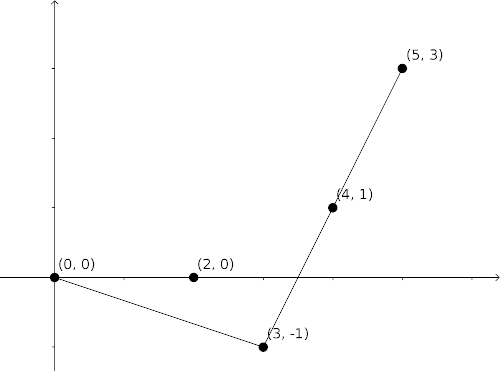
\includegraphics[scale=2.5]{/home/carlo/Tesi/images/figure_4_1}
				\caption{Newton polygon of $f(X) \in \Q_3[X]$}
				\label{figure:figure4.1}
			\end{figure}
		\end{example}
		Let's introduce some basic terms we'll adopt from now on.
		\begin{defn}
			The \emph{vertices} of the Newton polygon are the points $\left(i_j, \ord a_{i_j}\right)$ where the slope changes, the \emph{segments} of the Newton polygon are the segments joining one vertex to the next one; if a segment joins $(i, m)$ to $(i', m')$ its slope is $\tfrac{m' - m}{i' -i}$ and its length is $i' - i$, i.e. the length of its projection onto the horizontal axis.
		\end{defn}
		We have defined the Newton polygon only for a polynomial with constant term $1$, but this doesn't cause loss of generality because the main use of the Newton polygon is to characterize zeroes (and radius of convergence) of $f(X)$. Given a generic $g(X) \in \Cp[X]$ we can write:
		\[
			g(X) = b_kX^k + \dots + b_nX^n = b_k\cdot X^k \cdot \left(1 + \frac{b_{k+1}}{b_k}X + \dots + \frac{b_n}{b_k}X^{n-k}\right) =: b_k \cdot X^k \cdot f(X)
		\]
		and we can study $f(X)$, which satisfies our initial hypothesis.	Before proving our main result about the Newton polygon for polynomials, let's recall what symmetric polynomials are.
		\begin{defn}
			Let $K$ be a commutative ring with unit, $\underline{X} := (X_1, \dots, X_n)$ and let $P(\underline{X}) \in K[\underline{X}]$ be a polynomial in $n$ variables. We say that $P(\underline{X})$ is symmetric if for every $\sigma \in S_n$ we have $P(X_{\sigma(1)}, \dots, X_{\sigma(n)}) = P(X_1, \dots, X_n)$, where $S_n$ is the symmetric group of $n$ elements. \newline
			The symmetric polynomials $\left\{e_i(\underline{X}) : i \in \{0, 1, \dots, n\}\right\}$ defined by
			\begin{gather*}
				e_0(\underline{X}) = 1,\\
				e_k(\underline{X}) = \sum_{1 \leq i_1 < \dots < i_k \leq n} X_{i_1}X_{i_2}\dots X_{i_k}
			\end{gather*}
			are the \emph{elementary symmetric polynomials}.
		\end{defn}
		It is well known that the symmetric polynomials in $n$ variables form a subring $K[\underline{X}]^{S_n}$ and if $P(\underline{X})$ is symmetric then there exists $Q(\underline{Y}) \in K[\underline{Y}]$ such that $P(\underline{X}) = Q(e_1(\underline{X}), \dots, e_n(\underline{X}))$, i.e. the elementary symmetric polynomials ``generate'' all symmetric polynomials.
		It is easy to prove that if $f(X) \in K[X]$ is a monic polynomial of degree $n$ (here we add the hypothesis that $K$ is an integral domain, i.e. there are no divisors of zero) and all its roots are $\alpha_1, \dots, \alpha_n$ then
		\[
			f(X) = \prod_{j=1}^n \left(X - \alpha_j\right) = \sum_{j=0}^n (-1)^{n-j} \cdot e_{n-j}(\alpha_1, \dots, \alpha_n) \cdot X^j,
		\]
		which is a precise relation between the coefficients of $f$ and its roots. Finally we recall that if $f(X) = 1 + \sum_{i=1}^n a_iX^i \in K[X]$ has degree $n$ (here $K$ is a field) and $\alpha_1, \dots, \alpha_n$ are all of its roots, we can write
		\[
		f(X) = \prod_{j=1}^n \left(1 - \frac{X}{\alpha_j}\right) = \sum_{j=0}^n (-1)^j \cdot e_j\left(\frac{1}{\alpha_1}, \dots, \frac{1}{\alpha_n}\right) \cdot X^j;
		\]
		in-fact $f(0) = 1$ and we can divide by $1 = (-1)^na_n\alpha_1\dots\alpha_n$ both sides of $f(X) = a_n(X - \alpha_1)\dots(X - \alpha_n)$.\newline
		We are ready to state and prove the following.
		\begin{thm}
			\label{thm:newton-polygon-polinomial-zeroes}
			Let $f(X) = 1 + \sum_{i=1}^n a_iX^i \in 1 + X\Cp[X]$ be a polynomial of degree $n$, let $\alpha_1, \dots, \alpha_n \in \Cp$ be all of its roots and $\lambda_i := \mathrm{ord}_p\,\left(1/\alpha_i\right)$. If $\lambda$ is a slope of the Newton polygon of $f$ with length $l$, it follows that precisely $l$ of the $\lambda_i$ are equal to $\lambda$. Vice-versa, if $\gamma$ is a \padic order of a reciprocal root then there is a segment of the Newton polygon with slope $\gamma$.
		\end{thm}
		\begin{proof}
			The last statement is trivial if we prove the first one: in-fact the total length of the Newton polygon is $n$ so we have already considered all the roots (counting multiplicity).\newline
			Let's suppose the $\alpha_i$ arranged so that $\lambda_1 \leq \lambda_2 \leq \dots \leq \lambda_n$. Let's suppose that $\lambda_1 = \lambda_2 = \dots = \lambda_r < \lambda_{r+1}$. We then claim that the first segment of the Newton polygon is the one joining $(0,0)$ to $(r, r\lambda_1)$. We know that $a_i = (-1)^i \cdot e_i\left(1/\alpha_1, \dots, 1/\alpha_n\right)$ and, recalling how the $i$-th elementary symmetric polynomial is defined (sum of all possible products of $i$ different variables) and that $\ord(x + y) \geq \min\{\ord(x),\ord(y)\}$, we obtain 
			\[
			\ord(a_i) \geq i\lambda_1,
			\]
			which means that the point $(i, \ord(a_i))$ is on or above the line joining $(0,0)$ to $(r, r\lambda_1)$. Let's now consider $a_r$: only one of the products of $r$ of the $1/\alpha_i$ has \padic order $r\lambda_1$ and it is exactly $1/(\alpha_1 \dots \alpha_r)$, while all the other products have bigger \padic order since they must include at least one $1/\alpha_i$ with $i > r$. Then, by the isosceles triangle principle, $\ord(a_r) = r\lambda_1$. Finally, let's consider $a_i$ with $i > r$: for the same reasoning as before we have $\ord(a_i) > i\lambda_1$. \newline
			All these considerations means exactly that the first segment of the Newton polygon is the one joining $(0,0)$ and $(r, r\lambda_1) = (r, \lambda_1 + \dots + \lambda_r)$. Now, if we have $\lambda_s < \lambda_{s+1} = \dots = \lambda_{s+t} < \lambda_{s+t+1}$ the line joining $(s, \lambda_1 + \dots + \lambda_s)$ to $(s+t, \lambda_1 + \dots + \lambda_s + t\lambda_{s+1})$ is a segment of the Newton polygon. The proof is very similar: if $s \leq i$ then $\ord(a_i) \geq \lambda_1 + \dots + \lambda_s + (i-s)\lambda_{s+1}$, since this is the minimum \padic order in $e_i\left(1/\alpha_1, \dots, 1/\alpha_n\right)$, reached for example by $1/(\alpha_1\dots\alpha_i)$, $\ord(a_{s+t}) = \lambda_1 + \dots + \lambda_s + t\lambda_{s+1}$ by the isosceles triangle principle and if $i > s+t$ then $\ord(a_i) > \lambda_1 + \dots +\lambda_s + (i - s)\lambda_{s+1}$ since we have to choose at least one $1/\alpha_j$ with $j > s+t$.
		\end{proof}
		This theorem, in other words, says that the slopes of the Newton polygon of $f(X)$ are counting with multiplicity the \padic orders of the reciprocal roots of $f(X)$. The aim of the rest of this chapter will be to extend this result to formal power series, but we'll need to do a little more work before. 
	\section{Newton polygons for power series}
		The definition of the Newton polygon for $f(X) \in 1 + X\Cp\ser{X}$ is the same of \cref{defn:newton-polygon-polynomials}: it is the inferior convex hull of all the points in $\Gamma$ (which, this time, will be infinite). Sometimes we'll denote the Newton polygon of $f(X)$ by $\mathfrak{N}(f)$. From now on we'll only consider proper power series, i.e. we'll exclude the case in which $f(X)$ is a polynomial. We can distinguish three different kinds on Newton polygon.
		\begin{enumerate}[label=(\arabic*)]
			\label{enumerate:newton-polygon-types}
			\item We get infinitely many segments of finite length, for example the Newton polygon $f(X) = 1 + \sum_{i=1}^{+\infty} p^{i^2}X^i$ shown in \cref{figure:figure4.2}.
			\item At some point the line we're rotating simultaneously hits infinite points. In this case the Newton polygon has only a finite number of segments, the last one being infinitely long. An example is $f(X) = 1 + \sum_{i=1}^{+\infty} X^i$, whose Newton polygon is simply the horizontal axis.
			\item At some point the line we're rotating has not hit any point yet but it cannot rotate any farther without passing above some points. If this happens, we let the last segment of the Newton polygon have slope equal to the least upper bound of all possible slopes for which the line passes below all the points. A simple example is given by $f(X) = 1 + \sum_{i=1}^{+\infty} pX^i$, whose Newton polygon is the horizontal axis as shown in \cref{figure:figure4.3}.
		\end{enumerate}
		There is a degenerate case of type $(3)$: the vertical line through $(0,0)$ cannot be rotated at all without crossing above some points $(i, \ord a_i)$. An example of this possibility is given by $f(X) = \sum_{i=0}^{+\infty} \tfrac{X^i}{p^{i^2}}$, whose Newton polygon is shown in \cref{figure:figure4.3.1}.
		\begin{figure}
			\centering
			\subfloat[][Newton polygon of type 1 \label{figure:figure4.2}]{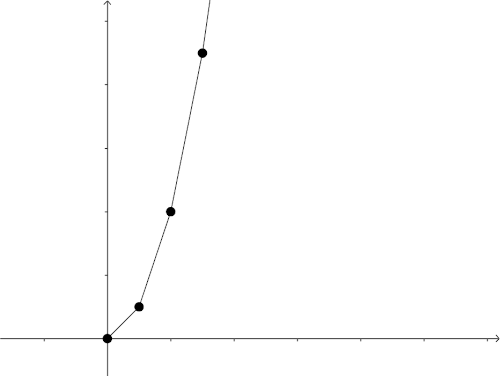
\includegraphics[scale=1.25]{/home/carlo/Tesi/images/figure_4_2}} \qquad \qquad
			\subfloat[][Newton polygon of type 3 \label{figure:figure4.3}]{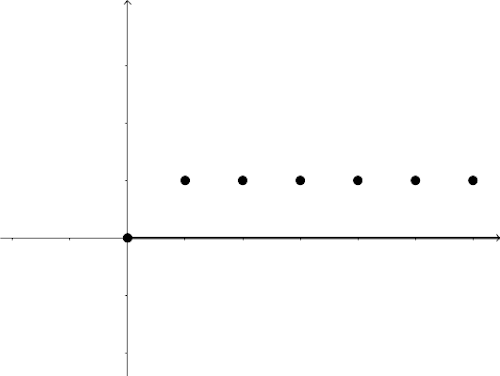
\includegraphics[scale=1.25]{/home/carlo/Tesi/images/figure_4_3}} \\
			\subfloat[][Degenerate Newton polygon \label{figure:figure4.3.1}]{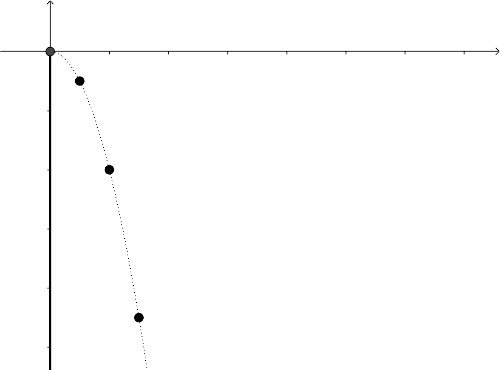
\includegraphics[scale=1.25]{/home/carlo/Tesi/images/figure_4_3_1}} \qquad \qquad
			\subfloat[][Newton polygon of $f(X)$ \label{figure:figure4.4}]{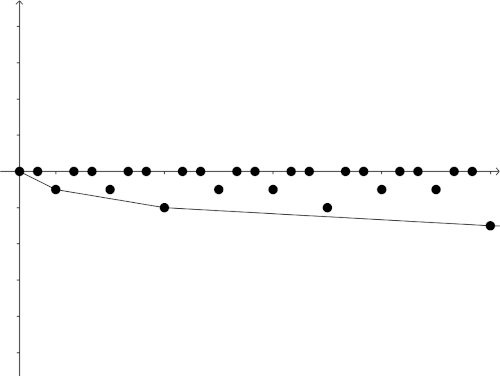
\includegraphics[scale=1.25]{/home/carlo/Tesi/images/figure_4_4}}	
			\caption{Various Newton polygons}		
		\end{figure}
		We'll exclude this case from our study since, as we'll prove in the next proposition, all such series have zero radius of convergence.
		\begin{prop}
			Let $f(X) = 1 + \sum_{i=1}^{+\infty} a_iX^i \in 1 + X\Cp\ser{X}$ be a power series whose Newton polygon is a degenerate case of type $(3)$, i.e. 
			\[
				\forall m \in \R \quad \exists i_m \in \N : \mathrm{ord}_p\, a_{i_m} < m \cdot i_m.
			\]
			Then the radius of convergence of $f$ is $0$.
		\end{prop} 
		\begin{proof}
			We just need to prove that $\limsup\, \pabs{a_n}^{1/n} = +\infty$. Let's define a subsequence of the coefficients $(a_{n_k})_{k \geq 1}$ by induction. We set $n_1 = i_{-1}$ so that $(n_1, \ord a_{n_1})$ lies below the line $y = -x$. Let's now consider the lines $\ell_1$, joining $(0, 0)$ to $(n_1, \ord a_{n_1})$, and $\ell_2$, with equation $y = -2x$: by hypothesis there must be an infinite number of points $(i, \ord a_i)$ lying below both of these two lines. Then there is at least one such point $(j, \ord a_j)$ with $j > n_1$ and we set $n_2 := j > n_1$. We can iterate this procedure (every time we choose $n_k > n_{k-1}$ such that $(n_k, \ord a_{n_k})$ lies below both $y = -kx$ and the line joining $(0,0)$ to $(n_{k-1}, \ord a_{n_{k-1}})$). We have obtained an increasing sequence $(n_k)_{k \geq 1} \subseteq \N$ such that
			\[
				\ord a_{n_k} < -k \cdot n_k \implies \pabs{a_{n_k}}^{1/n_k} > p^k.
			\]
			Using this subsequence we can conclude.
		\end{proof}
		From now on we'll always consider analytic functions with a non-trivial disc of convergence. Before proving general properties of the Newton polygon of analytic functions, let's consider a concrete example.
		\begin{example}
			Let's consider the function $f$ defined by
			\[
				f(X) = \sum_{n=0}^{+\infty} \frac{X^n}{n+1} = \frac{1}{X} \cdot \sum_{n=0}^{+\infty} \frac{X^{n+1}}{n+1} = -\frac{1}{X} \cdot \log_p(1 - X).
			\]
			Looking at the right member it's immediate to see that $f$ converges in $D(1^-)$. If we denote $\ell_i$ the segment joining $\left(p^i-1, -i\right)$ to $\left(p^{i+1}-1, -i-1\right)$ then it's easy to see that the Newton polygon of $f$ is the polygonal line $\bigcup_{i \in \N} \ell_i$ shown in \cref{figure:figure4.4} for $p=3$.
			Assuming that the power series analogue of \cref{thm:newton-polygon-polinomial-zeroes} holds, then, by looking at the Newton polygon of $f$, we would expect to find exactly $p^{i+1} - p^i$ roots having \padic order $1/\left(p^{i+1} - p^i\right)$ for every $i \in \N$ and no other roots. \newline 
			Let's prove this claim: let's fix $j \in \N$ and consider $x = 1 - \zeta$, where $\zeta \in \Cp$ is a primitive $p^{j+1}$-th root of $1$. Then we know by \cref{exercise:7-p.74} that $\ord x = 1/\left(p^{j+1} - p^j\right)$ and that $\log_p(1 - x) = 0$ by \cref{corollary:log-root-of-1} so $f(x) = 0$. Since there are exactly $p^{i+1} - p^i$ primitive roots of $1$, we have found all the predicted roots. Let's now prove that there are no other roots of $f$, i.e. any root is of the form $1 - \xi$ where $\xi$ is a primitive $p^k$-th root of $1$. Let $x \in D(1^-)$ be a root of $f$ and let
			\[
				x_j := 1 - (1 - x)^{p^j}
			\]
			for any $j \in \N$. Using Newton's binomial expansion we get
			\[
				\pabs{x_j} = \pabs{1 - (1 - x)^{p^j}} = \pabs{\sum_{i=1}^{p^j} \binom{p^j}{i} (-x)^i} \leq \pabs{x} < 1,
			\]
			which implies $x_j \in D(1^-)$ for every $j$. We claim that for any $M > 0$ we can find $j_m \in \N$ such that $\pabs{x_{j_m}}< M$. Fixed $M > 0$ we just need to find a $j$ such that
			\[
				\max_{1 \leq i \leq p^j} \pabs{\binom{p^j}{i}x^i} < M.
			\]
			Since $\pabs{x} < 1$ we can find $N \in \N$ such that if $n > N$ then $\pabs{\binom{p^j}{n}x^n} < M$. Now we just need to find a $j$ such that
			\[
					\max_{1 \leq i \leq N} \pabs{\binom{p^j}{i}x^i} < M.
			\]
			Writing $m := \max_{1 \leq i \leq N} (1/\pabs{i!}) > 0$ we have that
			\[
				\pabs{\binom{p^j}{i}} \leq \pabs{\frac{p^j}{i!}} \leq \pabs{p^j} \cdot m
			\]
			and we can conclude, since $\pabs{p^j} \to 0$ as $j \to +\infty$. Now let's consider $j \in \N$ such that $x_j \in D(r_p^-)$; thanks to \cref{prop:exp-and-log-inverse} we have
			\[
				1 - x_j = \exp_p(\log_p(1 - x_j)) =\exp_p\left(p^j\cdot \log_p(1 - x)\right) = \exp_p(0) = 1
			\]
			hence $(1 - x)^{p^j} = 1$ so that $x = 1 - \zeta$ where $\zeta$ is a $p^j$-th root of $1$ and it's one of the roots we already considered. \newline
			We have proved that, for this particular $f(X)$, the power series analogue of \cref{thm:newton-polygon-polinomial-zeroes} holds.
		\end{example}
		Let's now prove a simple but interesting result which explains how we can find the radius of convergence of a series just by looking at its Newton polygon.
		\begin{prop}
			\label{prop:newton-polygon-radius-convergence}
			Let $f(X) = 1 + \sum_{i=1}^{+\infty} a_iX^i \in 1 + X\Cp\ser{X}$ and let $b$ be the least upper bound of all slopes of the Newton polygon of $f$. Then the radius of convergence of $f(X)$ is $p^b$ (if $b=+\infty$ then $f$ converges everywhere).
		\end{prop}
		\begin{proof}
			Let's fix $x \in \Cp$ with $\pabs{x} < p^b$, i.e. $-b' := \ord x > -b$. Then $\ord(a_ix^i) = \ord a_i -ib'$ but, since $b' < b$, it's clear that sufficiently far out all the points $(i, \ord a_i)$ will lie arbitrarily far above $(i, b'i)$, see \cref{figure:figure4.5}. This means exactly $\lim_{i\to +\infty} \ord(a_ix^i) = +\infty$, i.e. $f(X)$ converges at $x$. \begin{figure}
				\centering
				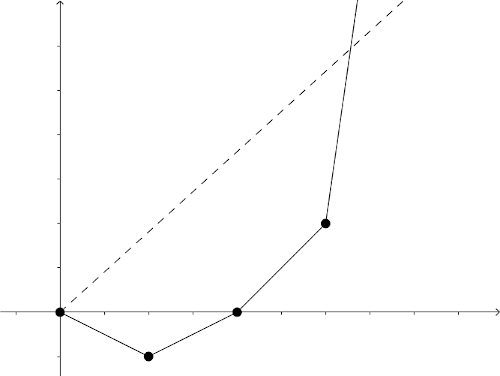
\includegraphics[scale=1.5]{/home/carlo/Tesi/images/figure_4_5}
				\caption{Case $\protect\pabs{x} < p^b$} % Workaround, it works
				\label{figure:figure4.5}
			\end{figure}
			Let's now consider the case $\pabs{x} > p^b$, i.e. $-b' := \ord x < -b$. Since $b' > b$ we find an infinite number of $i \in \N$ such that $\ord(a_ix^i) = \ord a_i - ib' < 0$ which implies that $f(X)$ does not converge at $x$. We can then conclude that the radius of convergence of $f$ is exactly $p^b$.
		\end{proof}
		Obviously this proposition doesn't tell us anything about the convergence of $f(X)$ at the radius of convergence, i.e. if $\pabs{x} = p^b$. 
		\begin{prop}
			\label{prop:newton-polygon-circonference-convergence}
			Let $f(X) = 1 + \sum_{i=1}^{+\infty} a_iX^i \in 1 + X\Cp\ser{X}$ be an analytic power series with radius of convergence $r=p^b$, where $b$ is the least upper bound of the slopes of the Newton polygon. Then $f(X)$ converges on $D(r)$ if and only if $\mathfrak{N}(f)$ is of type $(3)$ (see the beginning of \cref{enumerate:newton-polygon-types}) and $\lim_{i \to +\infty} d_i = +\infty$, where $d_i$ is the distance between $(i, \mathrm{ord}_p\, a_i)$ and the last line of $\mathfrak{N}(f)$.
		\end{prop}
		\begin{proof}
			If $b \notin \Q$ there's nothing to prove since no element of $\Cp$ can have order $b$; from now on we'll assume $b \in \Q$.
			First of all we prove that if the Newton polygon of $f$ is of type $(1)$ or $(2)$ then $f(X)$ does not converge if $\pabs{x} = p^b$. \newline 
			Let's first consider a Newton polygon of type $(1)$ and let $\Lambda$ be the set of all its slopes. Then $b = \sup \Lambda$ and if $b = +\infty$ there's nothing to prove. If $b < +\infty$ then there exists $y_0 \in \R$ such that $\ell\colon y = y_0 + bx$ is an ``asymptote'' of the Newton polygon, see \cref{figure:figure-extra-1} (the slopes are increasing and their $\sup$/$\lim$ is $b$). Then we can consider the vertices of the Newton polygon, indexed by $\left(i_j\right)_{j \in \N}$. It is clear that the distance $d_j$ between $\left(i_j, \ord a_{i_j}\right)$ and $\ell$ tends to $0$ and so does $\left(\ord a_{i_j} - i_jb\right)$, which is equal to $d_j/\cos(\arctan b)$ (if $b=0$ then it is equal to $d_j$). If $\pabs{x} = p^b$ then $\ord x = -b$ so $\ord(a_ix^i) = \ord a_i - ib$. We then conclude that $\ord(a_ix^i) \not\to +\infty$ when $i \to +\infty$, i.e. $f$ does not converge at $x$. 
			Instead if $f$ has a Newton polygon of type $(2)$ then $b$ is its final slope and, by definition, there are infinite points on this final segment. This means that if we call the final line $\ell\colon y_0 + bx$ then we can find an increasing subsequence $\left(i_j\right)_{j \in \N} \subseteq \N$ such that $\ord a_{i_j} = y_0 + i_jb$ so $\ord\left(a_{i_j}x^{i_j}\right) = y_0 \not\to +\infty$ and we can conclude that there's no convergence in $x$.\newline
			Let's now suppose that $\mathfrak{N}(f)$ is of type $(3)$ and $x \in \Cp$ with $\pabs{x} = p^b$. Then $f(X)$ converges in $x$ if and only if $\lim_{i \to +\infty} \ord\left(a_ix^i\right) = +\infty$; as before, with a little trigonometry, we have
			\begin{gather*}
				\ord\left(a_ix^i\right) = \ord a_i - ib = 
				\begin{cases}
					d_i, & \text{if $b=0$;} \\
					\frac{d_i}{\cos(\arctan b)}, & \text{otherwise;} 
				\end{cases}
			\end{gather*}
			and we can conclude (by hypothesis $\lim_{i \to +\infty} d_i = +\infty$). An example is $f(X) = 1 + \sum_{i=1}^{+\infty} 2^iX^{2^i} \in 1 + X\C_2\ser{X}$, whose Newton polygon is shown in \cref{figure:figure4.5.1}.
			\begin{figure}
				\centering
				\subfloat[][Newton polygon with an asymptote \label{figure:figure-extra-1}]{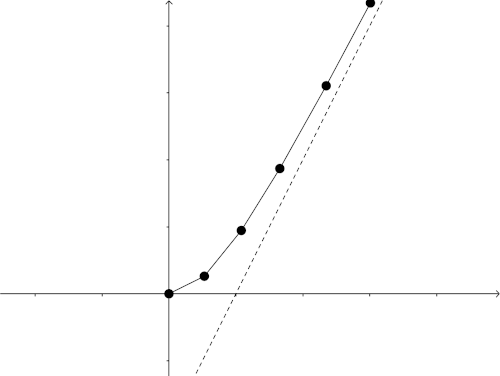
\includegraphics[scale=1.25]{/home/carlo/Tesi/images/figure_extra_1}} \qquad
				\subfloat[][Newton polygon with convergence at border \label{figure:figure4.5.1}]{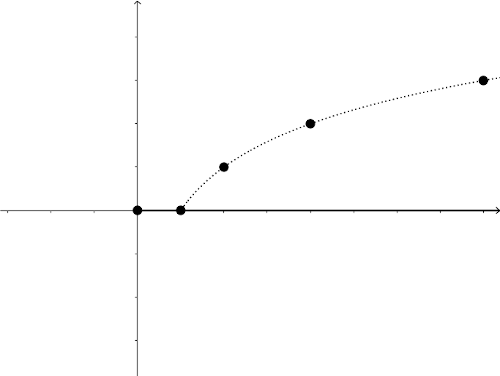
\includegraphics[scale=1.25]{/home/carlo/Tesi/images/figure_4_5_1}}
				\caption{Two other types of Newton polygons}
			\end{figure}
		\end{proof}
		Let's introduce a useful trick we'll often use in the next proofs.
		\begin{lemma}
			\label{lemma:newton-polygon-translation}
			Let $c \in \Cp^\times$ with $\mathrm{ord}_p\, c = \lambda$, $f(X) = 1 + \sum_{i=1}^{+\infty} a_iX^i \in 1 + X\Cp\ser{X}$ and $g(X) := f\left(X/c\right)$. Then the Newton polygon of $g$ is obtained subtracting the line $y = \lambda x$ to the Newton polygon of $f$.
		\end{lemma}
		\begin{proof}
			If we write $g(X) = 1 + \sum_{i=1}^{+\infty} b_iX^i$ then it's immediate that $b_i = a_i/\left(c^i\right)$ so $\ord b_i = \ord a_i - i\lambda$ and we can conclude.
		\end{proof}
		We'll now prove four technical lemmas we'll then use to prove our final result.
		\begin{lemma}
			\label{lemma:lemma6-p.102}
			Let $f(X) = 1 + \sum_{i=1}^{+\infty} a_iX^i \in 1 + X\Cp\ser{X}$ and suppose that $\lambda_1$ is the first slope of its Newton polygon. Let $c \in \Cp$ with $\mathrm{ord}_p\,c = \lambda \leq \lambda_1$ and assume that $f(X)$ converges on the closed disc $D(p^{\lambda})$ (this automatically happens if $\lambda < \lambda_1$ or if the Newton polygon has more than one segment). Let 
			\[
				g(X) = (1 - cX)f(X) \in 1 + X\Cp\ser{X}.
			\]
			Then $\mathfrak{N}(g)$ is obtained by joining $(0,0)$ to $(1, \lambda)$ and then translating $\mathfrak{N}(f)$ by $\vec{v} = (1, \lambda)$ ($1$ to the right and $\lambda$ upwards). If $\mathfrak{N}(f)$ has last slope $\lambda_f$ and $f(X)$ converges on $D(p^{\lambda_f})$ then $g(X)$ also converges on $D(p^{\lambda_f})$. Conversely, if $g(X)$ converges on $D(p^{\lambda_f})$ then so does $f(X)$.
		\end{lemma}
		\begin{proof}
			A graphic interpretation of the lemma can be found at \cref{figure:figure4.6}.
			\begin{figure}
				\centering
				\subfloat[][Newton polygon of $f_1(X)$]{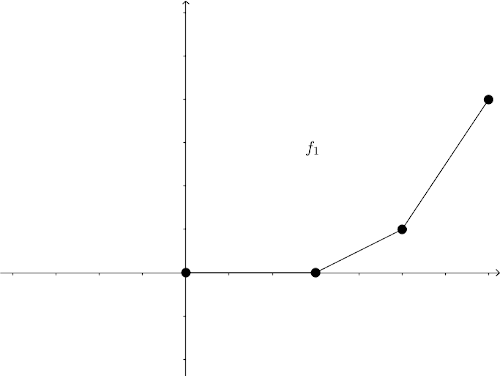
\includegraphics[scale=1.25]{/home/carlo/Tesi/images/figure_4_6_1}} \qquad \qquad \subfloat[][Newton polygon of $g_1(X)$]{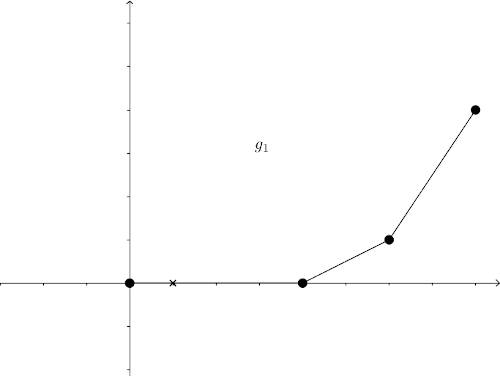
\includegraphics[scale=1.25]{/home/carlo/Tesi/images/figure_4_6_2}} \\
				\subfloat[][Newton polygon of $f(X)$]{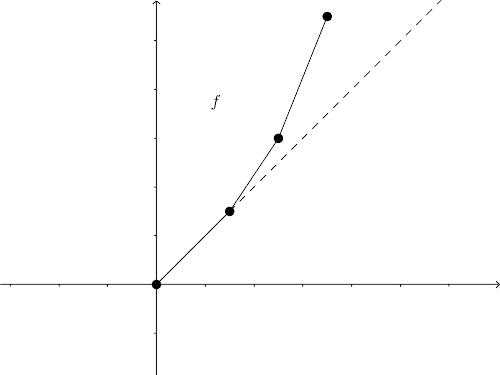
\includegraphics[scale=1.25]{/home/carlo/Tesi/images/figure_4_6_3}} \qquad \qquad
				\subfloat[][Newton polygon of $g(X)$]{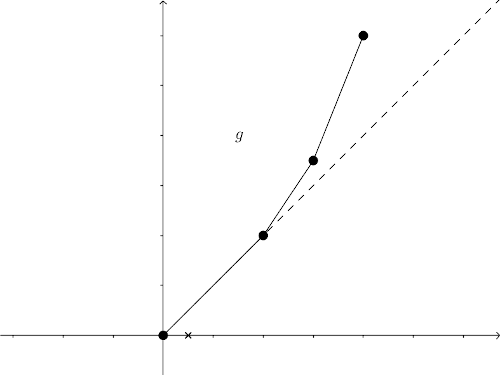
\includegraphics[scale=1.25]{/home/carlo/Tesi/images/figure_4_6_4}} 
				\caption{Example of \protect\cref{lemma:lemma6-p.102}}
				\label{figure:figure4.6}
			\end{figure}
			We can consider only the special case $c=1, \lambda = 0$. In-fact, let's suppose the lemma holds for this case and let $f(X)$ and $g(X)$ as in the statement. Then $f_1(X) := f\left(\tfrac{X}{c}\right)$ and $g_1(X) := (1 - X)f_1(X)$ satisfy our hypothesis (with the parameters $\underline{c}=1, \underline{\lambda} = 0, \underline{\lambda_1} = \lambda_1 - \lambda$, by \cref{lemma:newton-polygon-translation}). Thus, since we're assuming the lemma to be true if $c=1$, we know the shape of the Newton polygon of $g_1(X)$ (and the convergence of $g_1(X)$ on $D(p^{\lambda_f - \lambda})$ when $f$ converges on $D(p^{\lambda})$). Now, $g(X) = g_1(cX)$ so,  using again \cref{lemma:newton-polygon-translation}, we obtain the desired information about the Newton polygon of $g(X)$ (and the desired convergence, which is immediate). So we can just prove the lemma when $c = 1$.\newline
			If $g(X) = 1 + \sum_{i=1}^{+\infty} b_iX^i$ then, since by definition $g(X) = (1 - X)f(X)$, we have $b_{i+1} = a_{i+1} - a_i$ for $i \geq 0$ (clearly $a_0 = 1$). Then
			\begin{equation*}
				\ord b_{i+1} \geq \min\left\{\ord a_{i+1}, \ord a_i \right\} \tag{$\star$}
			\end{equation*}
			and the equality holds when $\ord a_{i+1} \neq \ord a_i$. It is easy to see that both $(i, \ord a_i)$ and $(i, \ord a_{i+1})$ lie on or above the Newton polygon of $f(X)$ and so does $(i, \ord b_{i+1})$, by $(\star)$. If $(i, \ord a_i)$ is a vertex then necessarily $\ord a_{i+1} > \ord a_i$ so $\ord b_{i+1} = \ord a_i$. This means exactly that the Newton polygon of $g(X)$ has the shape described in the lemma, as far as the last vertex of $f(X)$. If $\mathfrak{N}(f)$ is of type $(1)$ we can conclude here: there is no last vertex and no last slope. It remains only to show that when $\mathfrak{N}(f)$ has last slope $\lambda_f$ then also $\mathfrak{N}(g)$ does and if $f(X)$ converges on $D(p^{\lambda_f})$ then so does $g(X)$. We already know $\ord b_{i+1} \geq \min\left\{\ord a_{i+1}, \ord a_i \right\}$ so $g(X)$ converges wherever $f(X)$ does; then if $\lambda_g$ is the least upper bound of the slopes of $\mathfrak{N}(g)$ we have $\lambda_g \geq \lambda_f$ (by \cref{prop:newton-polygon-radius-convergence}). We must only rule out the case $\lambda_g > \lambda_f$. If it were the case, then, for some large $i$, the point $(i+1, \ord a_i)$ would lie below $\mathfrak{N}(g)$ so we'd have $\ord b_j > \ord a_i$ for every $j  \geq i+1$ (this holds in this particular case where $\lambda = 0$ since $0 \leq \lambda_1 \leq \lambda_f < \lambda_g$). Using $j = i+1$ we obtain $\ord a_{i+1} = \ord a_i$ because $a_{i+1} = b_{i+1} + a_i$. Then, using $j = i+2$, we obtain $\ord a_{i+2} = \ord a_{i+1} = \ord a_i$ and so on for every $j$. This means $\ord a_j = \ord a_i$ for every $j \geq i$ and contradicts the assumed convergence of $f(X)$ on $D(1) \subseteq D(p^{\lambda_f})$. Then we must have $\lambda_g = \lambda_f$ and $\mathfrak{N}(g)$ is exactly of the predicted shape. This implies in particular that if $f(X)$ converges on $D(p^{\lambda_f})$ then so does $g(X)$ (see \cref{prop:newton-polygon-circonference-convergence}). The converse assertion, i.e. convergence of $g(X)$ implies convergence of $f(X)$, can be proved in an analogue way.
		\end{proof}
		\begin{lemma}
			\label{lemma:lemma7-p.103}
			Let $f(X) = 1 + \sum_{i=1}^{+\infty} a_iX^i \in 1 + X\Cp\ser{X}$ have Newton polygon with first slope $\lambda_1$. Let's assume that $f(X)$ converges on $D\left(p^{\lambda_1}\right)$ and that the line $\ell\colon y = \lambda_1x$ actually passes through a point $(i, \mathrm{ord}_p\, a_i)$ with $i \geq 1$ (both of these conditions are automatically satisfied if $\mathfrak{N}(f)$ has more than one slope). Then there exists an $x \in \Cp$ for which $\mathrm{ord}_p\, x = -\lambda_1$ and $f(x) = 0$.
		\end{lemma}
		\begin{proof}
			Let's first consider the case $\lambda_1 = 0$ and then reduce the general case to this one. If $\lambda_1 = 0$ we have $\ord a_i \geq 0$ for every $i \in \N$ and $\lim_{i \to +\infty} \ord a_i = +\infty$ since $f(X)$ converges on $D(1)$. Let $N := \max \left\{i \in \N^\times : \ord a_i=0 \right\}$ and let $f_n(X) := 1 + \sum_{i=1}^n a_iX^i \in 1 + X\Cp[X]$. By \cref{thm:newton-polygon-polinomial-zeroes}, if $n \geq N$ then the polynomial $f_n(X)$ has precisely $N$ roots with \padic order $0$, let them be $x_{n, 1}, \dots, x_{n, N}$ (it's immediate that $\mathfrak{N}(f_n)$ has a first segment with slope $0$ and length $N$). Let's define a sequence: $x_N := x_{N, 1}$ and, for $n \geq N$, $x_{n+1} := x_{n+1, i}$ where $i$ is such that  $\pabs{x_{n+1, i} - x_n}$ is minimal. We claim that $\left(x_n\right)_{n \geq N} \subseteq \Cp$ is Cauchy and its limit $x$ is the desired root of $f$. If $S_n$ denotes the set containing the roots of $f_n(X)$, counted with multiplicity, for $n \geq N$ we have
			\[
				\pabs{f_{n+1}(x_n) - f_n(x_n)} = \pabs{f_{n+1}(x_n)} = \prod_{\alpha \in S_{n+1}} \pabs{1 - \frac{x_n}{\alpha}}
			\]
			where we used $f_n(x_n) = 0$ and $f_{n+1}(X) = \prod_{\alpha \in S_{n+1}} \left(1 - \tfrac{X}{\alpha}\right)$. It's clear that if $\alpha \in S_{n+1}$ then $\ord \alpha \leq 0$: in-fact we cannot have $\ord \alpha > 0$ and $f_{n+1}(\alpha) = 0$ by the isosceles triangle principle (recall that $\ord a_i \geq 0$). Now if $\alpha \in S_{n+1}$ has $\ord \alpha < 0$ then $\pabs{1 - \tfrac{x_n}{\alpha}} = 1$, since $\pabs{x_n} = 1$. Then we can write
			\[
				\pabs{f_{n+1}(x_n) - f_n(x_n)} = \prod_{i=1}^N \pabs{1 - \frac{x_n}{x_{n+1, i}}} = \prod_{i=1}^N \pabs{x_{n+1, i} - x_n} \geq \pabs{x_{n+1} - x_n}^N,
			\]
			by the choice of $x_{n+1}$. We have obtained
			\[
				\pabs{x_{n+1} - x_n}^N \leq \pabs{f_{n+1}(x_n) - f_n(x_n)} = \pabs{a_{n+1}x_n^{n+1}} = \pabs{a_{n+1}} 
			\]
			so $\lim_{n \to +\infty} \pabs{x_{n+1} - x_n}^N = 0$ (by hypothesis $\lim_{n \to +\infty} \pabs{a_{n+1}} = 0$) and we have proved that $\left(x_n\right)_{n \geq N}$ is Cauchy (see \cref{lemma:cauchy-sequence-ultrametric}). Since $\Cp$ is complete there exists $x := \lim_{n \to +\infty} x_n$ and, by continuity of $\pabs{\ }$, we have $\pabs{x} = 1$. It's clear that for any $y \in D(1)$ we have $\lim_{n \to +\infty} f_n(y) = f(y)$ (the \padic absolute value of the difference tends to zero) so we have $f(x) = \lim_{n \to +\infty} f_n(x)$. Now,
			\[
				\pabs{f_n(x)} = \pabs{f_n(x) - f_n(x_n)} = \pabs{x - x_n}\cdot\pabs{\sum_{i=1}^n a_i\frac{x^i - x_n^i}{x - x_n}} \leq \pabs{x - x_n}
			\]
			because $\pabs{a_i} \leq 1$ and $\pabs{\tfrac{x^i - x_n^i}{x - x_n}} = \pabs{x^{i-1} + x^{i-2}x_n + \dots + x_n^{i-1}} \leq 1$. Hence we can conclude that $f(x) = \lim_{n \to +\infty} f_n(x) = 0$ and we have proved the lemma if $\lambda_1 = 0$.\newline
			The general case follows easily. Let $\pi \in \Cp$ be any number with $\ord \pi = \lambda_1$. Clearly such a $\pi$ exists: for example, if $(i, \ord a_i)$ lies on $y=\lambda_1x$ and $i \geq 1$ (such a point exists by assumption) then $\pi$ can be any $i$-th root of $a_i$ (recall that $\Cp$ is algebraically closed). Now let $g(X) := f\left(X/\pi\right)$; it's clear by \cref{lemma:newton-polygon-translation} that $g(X)$ satisfies the conditions of the lemma with $\lambda_1 = 0$. Then we already 
			know that there exists $x_0$ with $\ord x_0 = 0$ such that $g(x_0) = 0$. Then if $x = x_0/\pi$ we have $\ord x = -\lambda_1$ and $f(x) = f\left(x_0/\pi\right) = g(x_0) = 0$.
		\end{proof}
		\begin{lemma}
			\label{lemma:lemma8-p.105}
			Let $f(X) = 1 + \sum_{i=1}^{+\infty} a_iX^i \in 1 + X\Cp\ser{X}$ and let $\alpha \in \Cp$ such that $f(\alpha) = 0$. Let $g(X)$ be obtained by dividing $f(X)$ by $1 - \tfrac{X}{\alpha}$. Then $g(X)$ converges on $D(\pabs{\alpha})$.
		\end{lemma}
		\begin{proof}
			First of all, let's observe that $\alpha \neq 0$ and that dividing $f(X)$ by $1 - \tfrac{X}{\alpha}$ is the same thing of multiplying $f(X)$ by the geometric series $\sum_{i=0}^{+\infty} \left(\tfrac{X}{\alpha}\right)^i$. Let's write $g(X) = 1 + \sum_{i=1}^{+\infty} b_iX^i$ and let $f_n(X) := 1 + \sum_{i=1}^n a_iX^i$ be the $n$-th partial sum of $f(X)$. By an easy computation we infer that
			\[
				b_i = \sum_{j=0}^i \frac{a_j}{\alpha^j}
			\]
			where we set $a_0 = 1$. Then it's easy to see that
			\[
				b_i\alpha^i = f_i(\alpha)
			\]
			hence $\pabs{b_i\alpha^i} = \pabs{f_i(\alpha)} \to 0$ as $i \to +\infty$, since $f(\alpha) = 0$ and $f(x) = \lim_{n \to +\infty}f_n(x)$ wherever $f$ converges. This means exactly that $g(X)$ converges on $D(\pabs{\alpha})$.
		\end{proof}
		\begin{lemma}
			\label{lemma:order-zeroes-function}
			Let $f(X) = 1 + \sum_{i=1}^{+\infty} a_iX^i \in 1 + X\Cp\ser{X}$ such that $\lambda$ is the first slope of $\mathfrak{N}(f)$ and $f$ converges on some disc $D$. If $\alpha \in D$ is a root of $f$, i.e. $f(\alpha) = 0$, then $\mathrm{ord}_p\, \alpha \leq -\lambda$. If $\lambda$ is the only slope of $\newt{f}$ and no point of $\newt{f}$ lies on $y=\lambda x$, then $\mathrm{ord}_p\,\alpha < -\lambda$.
		\end{lemma}
		\begin{proof}
			Let's suppose that $\alpha \in D$ is such that $\ord \alpha = -\lambda' > -\lambda$. We have
			\[
				\ord(a_i\alpha^i) = \ord a_i -i\lambda' > \ord a_i -i\lambda \geq 0,
			\]
			where we used that all the points $(i, \ord a_i)$ lie on or above the line $y=\lambda x$ (by definition of Newton polygon). Then we have $\ord 1 = 0$ and $\ord(a_i\alpha^i) > 0$ for $i \geq 1$ and so $\alpha$ cannot be a root of $f$. The last statement can be proved with an analogue reasoning.
		\end{proof}
		Finally we are ready to prove the main theorem of this section which will imply, as a corollary, the power series analogue of \cref{thm:newton-polygon-polinomial-zeroes}.
		\begin{thm}[\padic Weierstrass Preparation Theorem]
			\label{thm:weierstrass-padic-preparation}
			Let $f(X) = 1 + \sum_{i=1}^{+\infty} a_iX^i \in 1 + X\Cp\ser{X}$ converge on $D(p^{\lambda})$. Let $N$ be the total horizontal length of all segments in $\mathfrak{N}(f)$ having slope less or equal to $\lambda$ if this length is finite $($i.e. if $\mathfrak{N}(f)$ hasn't an infinitely long last segment of slope $\lambda)$. On the other hand, if the Newton polygon of $f$ has last slope $\lambda$, then let $N$ be the greatest index $i$ such that $(i, \ord a_i)$ lies on that final segment $($there must be such a final index since $f$ converges on $D(p^{\lambda}))$. Then there exists a polynomial $h(X) \in 1 + X\Cp[X]$ of degree $N$ and a power series $g(X) = 1 + \sum_{i=1}^{+\infty} b_iX^i$, which converges and is non-zero on $D(p^{\lambda})$, such that
			\[
				h(X) = f(X) \cdot g(X).
			\]
			The polynomial $h(X)$ is uniquely determined by these properties and $\mathfrak{N}(h)$ coincides with $\mathfrak{N}(f)$ up to $x = N$.
		\end{thm}
		\begin{proof}
			We use induction on $N$. Let's first consider the basic case $N = 0$, where the first slope of $\mathfrak{N}(f)$ is greater or equal to $\lambda$. In this case it's evident that we can assume $\lambda \in \Q$ without loss of generality. We have to show that $g(X) = 1/f(X)$ converges and is non-zero on $D(p^{\lambda})$ (recall that any power series with a non-zero constant term is invertible). We can only consider the special case $\lambda = 0$. In-fact, let $f(X) \in 1 + X\Cp\ser{X}$ converge on $D(p^{\lambda})$: we can choose $c \in \Cp$ with $\ord c = \lambda$ using \cref{prop:qpa-every-order} (we assumed $\lambda \in \Q$) and then define $\tilde{f}(X) := f\left(\tfrac{X}{c}\right)$. Now, $\tilde{f}$ converges on $D(1)$ and if $\lambda = 0$ then $N = 0$, i.e. the first slope of its Newton polygon is greater or equal to $0$ by \cref{lemma:newton-polygon-translation}. So, assuming the theorem holds when $N = \lambda = 0$ we infer that there exists $\tilde{g}(X) \in 1 + X\Cp\ser{X}$ which converges and is non-zero on $D(1)$ such that $1 = \tilde{f}(X)\cdot\tilde{g}(X)$. Using $cX$ in place of $X$ we obtain $1 =f(X) \cdot \tilde{g}(cX)$ and it's immediate that $g(X) := \tilde{g}(cX)$ has all the desired properties. So we can only consider the special case $\lambda = 0$. Thus, we can suppose $\ord a_i > 0$ for every $i \in \N$ and $\lim_{i \to +\infty} \ord a_i = +\infty$ (we have convergence on $D(1)$). It's easy to obtain the following equality for the coefficients of $g(X) = 1/f(X)$:
			\[
				b_i = -\left(\sum_{j=1}^i b_{i-j}a_j \right),
			\]
			where we set $b_0 = 1$. From an easy induction on $i$ it follows that $\ord b_i > 0$ for $i \geq 1$. This implies that the first slope of $\mathfrak{N}(g)$ is greater than $0$ (or it's equal to $0$ but with no points on it) and, by \cref{lemma:order-zeroes-function}, we know that $g$ doesn't have roots on $D(1)$. Now it remains only to show that $g(X)$ actually converges on $D(1)$, i.e. that $\lim_{i \to +\infty} \ord b_i = +\infty$. Let's fix $M > 0$: we can find $m \in \N$ such that $i > m$ implies $\ord a_i > M$. Now if
			\[
				\epsilon := \min_{1 \leq j \leq m} \ord a_j> 0
			\]
			we claim that $i > nm$ implies $\ord b_i > \min\{M, n\epsilon\}$, from which it easily follows $\ord b_i \to +\infty$ as $i \to +\infty$. We'll prove this claim by induction on $n$. We have already proved the case $n = 0$. Now, let's suppose $n \geq 1$ and that the claim holds for $n - 1$; if $i > nm$ we have
			\[
				b_i = -\left(b_{i-1}a_i + \dots + b_{i-m}a_m + b_{i-(m+1)}a_{m+1} + \dots + a_1 \right).
			\]
			The terms $b_{i-j}a_j$ with $j > m$ have \padic order greater than $M$, while if $j \geq m$ we have $\ord(b_{i-j}a_j) \geq \ord b_{i-j} + \epsilon$ and, since $i - j > (n-1)m$, by inductive hypothesis we obtain
			\[	
				\ord(b_{i-j}a_j) \geq \ord b_{i-j} + \epsilon > \min\{M, (n-1)\epsilon\} + \epsilon.
			\]
			This proves our claim, hence the theorem when $N = 0$ (the statement about the Newton polygon here is trivial since $h(X) = 1$).\newline
			Now let's consider the general case with $N \geq 1$ and suppose that the theorem holds for $N - 1$. Let $\lambda_1 \leq \lambda$ be the first slope of $\mathfrak{N}(f)$; if it is the only slope then, since $N \geq 1$, there's at least one point on $y = \lambda_1x$. We can then use \cref{lemma:lemma7-p.103} to find $\alpha$ such that $f(\alpha) = 0$ and $\ord \alpha = -\lambda_1$. Let's define
			\[
				f_1(X) := \frac{f(X)}{1 - \frac{X}{\alpha}} = f(X) \cdot \sum_{j=0}^{+\infty} \left(\frac{X}{\alpha}\right)^j \in 1 + X\Cp\ser{X}.
			\]
			By \cref{lemma:lemma8-p.105}, $f_1$ converges on $D(p^{\lambda_1})$. Setting $c := \tfrac{1}{\alpha}$ we have $f(X) = (1 - cX)\cdot f_1(X)$. Let $\lambda_1'$ be the first slope of $\mathfrak{N}(f_1)$; it must necessarily be $\lambda_1' \geq \lambda_1$. In-fact $\lambda_1' < \lambda_1$ implies that $\mathfrak{N}(f_1)$ has more than one slope and that, by \cref{lemma:lemma7-p.103}, $f_1$ has a root with \padic order $-\lambda_1'$ and so does $f$, but this is impossible by \cref{lemma:order-zeroes-function} since $-\lambda_1' > -\lambda_1$. We can now apply \cref{lemma:lemma6-p.102}, with parameters $\underline{f} = f_1, \underline{g} = f, \underline{\lambda} = \lambda_1, \underline{\lambda_1} = \lambda_1'$ and we get that $\mathfrak{N}(f_1)$ is obtained translating $\mathfrak{N}(f) \setminus \ell((0,0), (1, \lambda_1))$ by $\vec{v} = (-1, -\lambda_1)$, where $\ell(P, Q)$ is the segment joining $P$ to $Q$. We claim that $f_1$ converges on $D(p^{\lambda})$: if $\lambda$ isn't the final slope of $\mathfrak{N}(f)$ then it's trivially true, otherwise \cref{lemma:lemma6-p.102} tells us that when $\mathfrak{N}(f)$ has last slope $\lambda$ and $f$ converges on $D(p^{\lambda})$ then so does $f_1$. Thus, $f_1$ satisfies all the conditions of the theorem with $N-1$ instead of $N$ (recall that, to obtain $\mathfrak{N}(f_1)$, we removed a segment with slope $\lambda_1 \leq \lambda$ and with length $1$ from $\mathfrak{N}(f)$). By inductive hypothesis we can find $h_1(X) \in 1 + X\Cp[X]$ of degree $N-1$ and a series $g(X) \in 1 + X\Cp\ser{X}$, convergent and non-zero on $D(p^{\lambda})$, such that
			\[
				h_1(X) = f_1(X) \cdot g(X).
			\]
			Multiplying both sides by $(1 - cX)$ and setting $h(X) := (1 - cX)h_1(X)$ we obtain
			\[
				h(X) = f(X) \cdot g(X),
			\]
			where $h$ and $g$ have the desired properties. Let's also observe that $\mathfrak{N}(h_1)$ coincides with $\mathfrak{N}(f_1)$ up to $x = N-1$ and that, since $h(X) = (1 - cX)h_1(X)$, $\mathfrak{N}(h)$ is obtained joining $(0,0)$ to $(1, \lambda_1)$ and then translating $\mathfrak{N}(h_1)$. Then it's clear that $\mathfrak{N}(h)$ will coincide with $\mathfrak{N}(f)$ up to $x = N$.\newline 
			Now we have only to prove the uniqueness of $h(X)$ (we have only proved its existence).
			Let's suppose that $\tilde{h}(X) \in 1 + X\Cp[X]$ is another polynomial of degree $N$ such that \[
				\tilde{h}(X) = f(X) \cdot g_1(X),
			\]
			where $g_1(X) \in 1 + X\Cp\ser{X}$ converges and is non-zero on $D(p^{\lambda})$. We have
			\[
				\tilde{h}(X)\cdot g(X) = f(X)\cdot g(X) \cdot g_1(X) = h(X) \cdot g_1(X). \tag{$*$}
			\]
			To prove uniqueness it suffices to show that $(*)$ implies that $h$ and $h_1$ have the same roots with the same multiplicities (they both have constant term $1$). The case $N=1$ is trivial. Let's now consider $N > 1$. The polynomial $h(X)$ is the one we built before so we already know that $\mathfrak{N}(h)$ coincides with $\mathfrak{N}(f)$ up to $x = N$. Using \cref{thm:newton-polygon-polinomial-zeroes}, this means that every root of $h(X)$ is in $D(p^{\lambda})$ (by assumption all the slopes of $\mathfrak{N}(h)$ are less or equal to $\lambda$). Let $\alpha \in \Cp$ be a root of $h(X)$. Since $\alpha \in D(p^{\lambda})$ we can compute $g(\alpha)$ and $g_1(\alpha)$ and, by hypothesis, they're not zero. So $\alpha$ must also be a root of $\tilde{h}(X)$. Let's define 
			\[
				\tilde{k}(X) := \frac{\tilde{h}(X)}{1 - \frac{X}{\alpha}}, \qquad k(X) := \frac{h(X)}{1 - \frac{X}{\alpha}};
			\]
			they're two polynomials in $1 + X\Cp[X]$ of degree $N - 1$ satisfying $\tilde{k}(X)\cdot g(X) = k(X)\cdot g_1(X)$. We can repeat this process with every other root of $h(X)$ and, at the end, both polynomials will be $1$ so we have proved uniqueness.
		\end{proof}
		This is a very powerful theorem, with a lot of interesting corollaries.
		\begin{corollary}
			\label{corollary:newton-polygon-zeroes}
			If a segment of the Newton polygon of $f(X) \in 1 + X\Cp\ser{X}$ has finite length $N$ and slope $\lambda$, then there are exactly $N$ values of $x$ (counting multiplicity) for which $f(x) = 0$ and $\mathrm{ord}_p\, x = -\lambda$.
		\end{corollary}
		\begin{proof}
			It is an immediate application of \cref{thm:weierstrass-padic-preparation} and \cref{thm:newton-polygon-polinomial-zeroes}. 
		\end{proof}
		\begin{example}
			We can use the Newton polygon to study the exact region of convergence of $\E_p(X)$, the Artin-Hasse exponential (see \cref{defn:artin-hasse}). We already know, by \cref{prop:artin-hasse-formula} and \cref{prop:artin-hasse-formula}, that
			\[
				\E_p(X) = \exp_p\left(\sum_{i=0
				}^{+\infty} \frac{X^{p^i}}{p^i}\right)
			\]
			and that $\E_p(X)$ converges on $D(1^-)$. We'll show that this is the exact region of convergence, i.e. that $\E_p(X)$ doesn't converge if $\pabs{x} = 1$. Let's define
			\[
				f(X) = \sum_{i=0}^{+\infty} \frac{X^{p^i -1}}{p^i} \in 1 + X\Cp\ser{X},
			\]
			so that $\E_p(X) = \exp_p(X \cdot f(X))$. Now, $\E_p(X)$ converges at $x \in \Cp$ if and only if $x\cdot f(x) \in D(r_p^-)$. We'll show that $f(X)$ doesn't even converge if $\pabs{x} = 1$. Writing $f(X) = 1 + \sum_{n=1}^{+\infty} a_iX^i$, it's immediate that
			\begin{gather*}
				(i, \ord a_i) =
				\begin{cases}
					\left(p^k - 1, -k\right), & \text{if $\exists k \in \N$ such that $i = p^k - 1$;} \\
					(i, 0), & \text{otherwise;}
				\end{cases}.
			\end{gather*}
			If $\ell_i$ is the segment joining $\left(p^i-1, -i\right)$ to $\left(p^{i+1}-1, -i-1\right)$ then we have $\mathfrak{N}(f) = \bigcup_{i \in \N} \ell_i$ (see \cref{figure:figure-extra-2} for $p=2$). It is clearly a type $(1)$ polygon (infinite number of finite segments). The segment $\ell_i$ has slope $\lambda_i =- \tfrac{1}{p^i(p - 1)} < 0$ and we have $\lim_{i \to +\infty} \lambda_i = 0$. This proves that $0$ is the least upper bound of all slopes of $\mathfrak{N}(f)$ so, using \cref{prop:newton-polygon-radius-convergence}, we can conclude: the radius of convergence of $f$ is $1 = p^0$ and we cannot have convergence ``at the border'', since we would need a type $(3)$ polygon.
			\begin{figure}
				\centering
				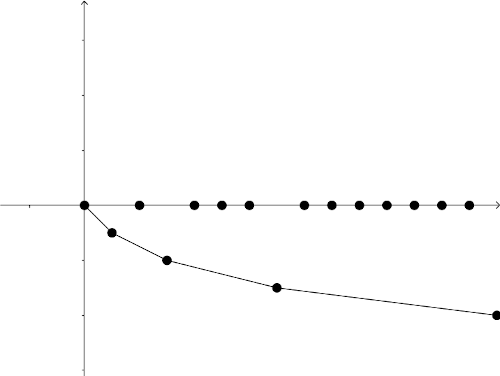
\includegraphics[scale=1.5]{/home/carlo/Tesi/images/figure_extra_2}
				\caption{Newton polygon of $f(X)$ for $p=2$}
				\label{figure:figure-extra-2}
			\end{figure}
		\end{example}
		Finally, we'll show a nice application of \cref{thm:weierstrass-padic-preparation}, which will imply the non-existence of a non-constant power series which converges on $\Cp$ and is never zero. This means exactly that we cannot have an exponential with the same properties of the classical one: in-fact in the classical case, if $h(X)$ is a convergent power series, then $e^{h(X)}$ is everywhere convergent and non-zero. We'll first need a technical lemma.
		\begin{lemma}
			\label{lemma:infinite-zeroes}
			Let $f(X)$ be a power series which converges on $D(p^{\lambda})$. If $f(X)$ has an infinite number of zeroes on $D(p^{\lambda})$ then $f(X)$ is identically zero.
		\end{lemma}
		\begin{proof}
			If $f(X) = 0$ there's nothing to prove, otherwise we can assume, by contradiction, $f(X) \in 1 + X\Cp\ser{X}$ (we can write $f(X) = a_dX^d \cdot g(X)$, where $d$ is such that $a_d$ is the first non-zero coefficient and study $g(X) \in 1 + X\Cp\ser{X}$). We can then apply \cref{thm:weierstrass-padic-preparation}, using $\lambda$, to obtain $N \in \N$, $h(X) \in 1 + X\Cp[X]$, a polynomial of degree $N$, and $g(X) \in 1 + X\Cp\ser{X}$, a power series convergent and non-zero on $D(p^{\lambda})$, such that
			\[
				h(X) = f(X) \cdot g(X).
			\]
			By hypothesis, $f(X)$ has infinite zeroes in $D(p^{\lambda})$ and, since $g(X)$ is never zero on $D(p^{\lambda})$, $h(X)$ must have infinite zeroes on $D(p^{\lambda})$. But $h(X)$ is a non-zero polynomial of degree $N$ so it cannot have infinite zeroes, and this is a contradiction. Thus the only possible case is $f(X) = 0$.
		\end{proof}
		\begin{prop}
			Let $f(X) = 1 + \sum_{i=1}^{+\infty} a_iX^i \in 1 + X\Cp\ser{X}$ be an everywhere convergent power series. For every $\lambda$, let $h_{\lambda}(X)$ be the polynomial obtained applying \cref{thm:weierstrass-padic-preparation}. Then $h_{\lambda} \to f$ as $\lambda \to +\infty$ (i.e., each coefficient of $h_{\lambda}$ converges to the corresponding coefficient of $f$). In particular, if $f$ is not a polynomial, then its zeroes are $(r_n)_{n \geq 1}$ (i.e. they're countable infinite) and 
			\[
				f(X) = \prod_{i=1}^{+\infty} \left(1 - \frac{X}{r_i}\right).
			\] 
		\end{prop}
		\begin{proof}
			If $f(X)$ is a polynomial, then the statement is trivial. From now on we'll consider $f(X)$ to be a proper power series. It's clear that such an $f$ must have a type $(1)$ Newton polygon. Let $(\lambda_n)_{n \geq 1}$ be the slopes of $\mathfrak{N}(f)$ (clearly we consider them in order, i.e. such that $\lambda_1 < \lambda_2 < \dots < \lambda_n < \dots$). Since $f(X)$ converges everywhere, by \cref{prop:newton-polygon-radius-convergence} we must have $\lim_{n \to +\infty} \lambda_n = +\infty$. It is also clear that $f$ has a countable infinite set of zeroes (there's clearly no contradiction here, because the zeroes are in $\Cp$): in-fact, applying \cref{corollary:newton-polygon-zeroes}, we obtain that for any segment of $\mathfrak{N}(f)$ we have a finite number of zeroes (and clearly the segments of the Newton polygon are countable infinite). Let it be $(r_n)_{n \geq 1}$, where they're listed in such a way that the first ``cluster'' corresponds to slope $\lambda_1$, the second to slope $\lambda_2$ and so on. Applying \cref{thm:weierstrass-padic-preparation} with $\lambda = \lambda_n$ we obtain a polynomial $1 + X\Cp[X] \ni h_n(X) := h_{\lambda_n}(X)$ and a power series $g_n(X) \in 1 + X\Cp\ser{X}$, convergent and non-zero on $D(p^{\lambda_n})$, such that
			\[
				h_n(X) = f(X) \cdot g_n(X).
			\]
			Let's introduce some terminology:
			\begin{gather*}
				h_n(X) = 1 + \sum_{i=1}^{d_n} a_{n,i}X^i, \qquad g_n(X) = 1 + \sum_{i=1}^{+\infty} b_{n, i}X^i,
			\end{gather*}
			where we set $d_n := \deg h_n(X)$. By \cref{thm:weierstrass-padic-preparation} we know that $d_n$ is the total horizontal length of segments of $\mathfrak{N}(f)$ with slope less or equal to $\lambda_n$ and this also means that
			\[
				h_n(X) = \prod_{j=1}^{d_n} \left(1 - \frac{X}{r_j}\right). \tag{$*$}
			\]
			First of all, let's prove that the sequences $(a_{n,m})_{n \geq 1}$ are all Cauchy \emph{uniformly} in $m$, i.e. we'll find an upper bound which doesn't depend on $m$. 
			Let $k \in \N$ be such that $\lambda_1 < \dots < \lambda_k < 0 \leq \lambda_{k+1}$, i.e. the first $k$ slopes of $\mathfrak{N}(f)$ are negative. Let's consider $r_1, \dots, r_{d_k}$, all the roots of $f$ (they're not necessarily distinct) corresponding to the negative slopes of $\mathfrak{N}(f)$. Then $\pabs{1/r_i} = p^{\ord r_i} > 1$, for every $1 \leq 1 \leq d_k$. Instead, for any other root $r_m$ with $m > d_k$ we have $\pabs{1/r_m} \leq 1$, since it corresponds to a non-negative slope. Let's set $M := \pabs{1/r_1}\cdots\pabs{1/r_{d_k}}$ (if all slopes are non-negative we simply set $M = 1$). Recalling the relations between coefficients and reciprocal of roots (using elementary symmetric polynomials), for $n \geq k$, by $(*)$, we have
			\[
				a_{n, m} = (-1)^m \cdot e_m\left(\frac{1}{r_1}, \dots, \frac{1}{r_{d_k}}, \frac{1}{r_{d_k + 1}}, \dots, \frac{1}{r_{d_n}}\right).
			\]
			Since for any $j > d_k$ we have $\pabs{1/r_j} \leq 1$, it's easy to see that
			\[
				\pabs{a_{n,m}} \leq \pabs{1/(r_1 \cdots r_{d_k})} = M,
			\]
			for any $m \in \N$ and $n \geq k$. We have found a common upper bound for all the coefficients of all the polynomials $h_n(X)$ with $n \geq k$. Now we have
			\[
				h_{n+1}(X) = h_n(X) \cdot \prod_{j=d_n+1}^{d_{n+1}} \left(1 - \frac{X}{r_j}\right)
			\]
			so we obtain
			\[
				a_{n+1, m} = a_{n, m} + \sum_{j=1}^m (-1)^j\cdot a_{n, m-j}\cdot e_j\left(\frac{1}{r_{d_n + 1}}, \dots, \frac{1}{r_{d_{n+1}}}\right),
			\]
			where we set $a_{n, 0} = 1$. Since $\lim_{n \to +\infty} d_n = +\infty$ (by construction) we can choose a large enough $n$ such that $\lambda_{n+1} > 0$. Then, $\pabs{1/r_j} = p^{\ord r_j} = p^{-\lambda_{n+1}} < 1$ for any $d_n + 1 \leq j \leq d_{n+1}$. Now it's easy to see that 
			\begin{gather*}
				\forall\, j \in \N, \quad  \pabs{e_j\left(\frac{1}{r_{d_n + 1}}, \dots, \frac{1}{r_{d_{n+1}}}\right)} \leq \pabs{\frac{1}{r_{d_n + 1}}} = p^{-\lambda_{n+1}} \\
				\implies \pabs{a_{n+1, m} - a_{n,m}} = \max_{1 \leq j \leq m} \pabs{a_{n, m-j}\cdot e_j\left(\frac{1}{r_{d_n + 1}}, \dots, \frac{1}{r_{d_{n+1}}}\right) } \leq M \cdot  p^{-\lambda_{n+1}}.
			\end{gather*}
			Since  $\lim_{n \to +\infty} p^{-\lambda_{n+1}} = 0$, $(a_{n, m})_{n \geq 1}$ is Cauchy (see \cref{lemma:cauchy-sequence-ultrametric}). Let's observe that our bounds don't depend on $m$, i.e. $\pabs{a_{n+1, m} - a_{n, m}} \leq M\cdot p^{-\lambda_{n+1}}$ for any $m \in \N$ and $n \geq k$. Since $(\lambda_n)_{n \geq 1}$ is non-decreasing, for $m > n \geq k$ we obtain
			\[
				\pabs{a_{m, i} - a_{n, i}} \leq \max_{n \leq j < m}\pabs{a_{j+1, i} - a_{j,i}} \leq \max_{n \leq j < m} Mp^{-\lambda_{j+1}} = Mp^{-\lambda_{n+1}}.
			\]
				
			Now, we know that $g_n(X)$ converges and is non-zero on $D(p^{\lambda_n})$; this means exactly that, if $\gamma_n$ is the first slope of $\mathfrak{N}(g_n)$, then $\gamma_n > \lambda_n$. In-fact, $\gamma_n \leq \lambda_n$ would imply, by \cref{corollary:newton-polygon-zeroes}, the existence of $\alpha \in \Cp$ such that $\pabs{\alpha} = p^{\gamma_n} \leq p^{\lambda_n}$ such that $g(\alpha) = 0$ and this cannot be the case. From a geometrical point of view, this means that every point $(i, \ord b_{n,i})$ lies on or above the line $y = \gamma_n \cdot x$, i.e.
			\[
				\ord b_{n,i} \geq i \cdot \gamma_n.
			\]
	 		We have already proved that $\lim_{n \to +\infty} \lambda_n = +\infty$ so $\lim_{n \to +\infty} \gamma_n = +\infty$ and this implies $\lim_{n \to +\infty} \ord b_{n,i} = +\infty$, i.e. $\lim_{n \to +\infty} b_{n,i} = 0$ for every $i \geq 1$. Let's now come back to the relation $h_n(X) = f(X)\cdot g_n(X)$ and let's consider the single coefficients; we obtain 
			\begin{align*}
				a_{n, 1} &= b_{n,1} + a_1; \\
				a_{n, 2} &= b_{n,2} + a_1b_{n,1} + a_2; \\
				\vdots \\
				a_{n, m} &= b_{n, m} + \sum_{j=1}^{m-1} a_jb_{n, m-j} + a_m.
			\end{align*}
			Then, for any $m \geq 1$, we have $\lim_{n \to +\infty} a_{n, m} = a_m$. Let's fix $x \in D(1)$ and $\epsilon > 0$ and consider
			\begin{gather*}
				\pabs{f(x) - h_n(x)} = \pabs{\sum_{i=1}^{+\infty} (a_i - a_{n, i}) x^i} \leq \max\left\{\max_{1 \leq i \leq d_n} \pabs{a_i - a_{n,i}},\, \max_{i > d_n}\,\pabs{a_i} \right\}
			\end{gather*}
			where we set $a_{n, i} = 0$ if $i > d_n$. We already know $\lim_{n \to +\infty} d_n =+\infty$ and we know that $\lim_{i \to +\infty} \pabs{a_i} = 0$ since $f$ converges everywhere (see \cref{prop:summable_families}). Let's choose $n \in \N$ such that $i > d_n$ implies $\pabs{a_i} < \epsilon$. Now we have only to give an upper bound on the first term, but this is easy thanks to the bounds we proved before:
			\begin{gather*}
				\pabs{a_i - a_{n, i}} = \lim_{m \to +\infty} \pabs{a_{m, i} - a_{n, i}} \leq \lim_{m \to +\infty} Mp^{-\lambda_{n+1}} = Mp^{-\lambda_{n+1}} \\
				\implies \max_{1 \leq i \leq d_n} \pabs{a_i - a_{n,i}} \leq M\cdot p^{-\lambda_{n+1}}
			\end{gather*}
			and we can assume that $n \in \N$ is big enough such that $M\cdot p^{-\lambda_{n+1}} < \epsilon$ and $i > d_n$ implies $\pabs{a_i} < \epsilon$. Since $\epsilon$ is chosen arbitrarily, we conclude that if $x \in D(1)$ then
			\[
				f(x) = \lim_{n \to +\infty} h_n(x) = \lim_{n \to +\infty} \prod_{j=1}^{d_n} \left(1 - \frac{x}{r_j}\right) = \prod_{j=1}^{+\infty} \left(1 - \frac{x}{r_j}\right).
			\]
			Let's define $\ell(X) := \prod_{j=1}^{+\infty} \left(1 - \frac{X}{r_j}\right)$. It can be proved that $\ell(X) \in 1 + X\Cp\ser{X}$ exploiting the fact that $\lim_{n \to +\infty} \pabs{1/r_n} = 0$ and that its coefficient of $X^m$ is simply the sum of the series of all possible products of $m$ of the $-1/r_i$'s (which converges). Now, $\ell(X)$ converges on $D(1)$ because $\ell(x) = f(x)$ for any $x \in D(1)$. We can conclude that, in $\Cp\ser{X}$, we have
			\[
				f(X) = \ell(X) = \prod_{j=1}^{+\infty} \left(1 - \frac{X}{r_j}\right) 
			\]
			since $g(X) := f(X) - \ell(X)$ is a power series convergent on $D(1)$ with infinite zeroes and, by \cref{lemma:infinite-zeroes}, it must be $g(X) = 0$. 	
		\end{proof}
		This proposition resembles a lot the Weierstrass factorization theorem of complex analysis, although the \padic result is much more clean: there are no exponential factor in the product. One immediate implication is that any power series which converges everywhere and is never zero must be a constant: here is why we cannot have an exponential similar to the classic one, which converges everywhere, is never zero but isn't constant. Finally we can think as power series which converges everywhere simply as ``polynomials with infinite zeroes'', which can be factorized in the same exact way we factorize polynomials. 